\newpage
\section{Fast Reduction}

\begin{align*}
p_{256} &= 2^{256} - 2^{224} + 2^{192} + 2^{96} - 1 \\
0 &\equiv 2^{256} - 2^{224} + 2^{192} + 2^{96} - 1 \pmod{p_{256}} \\
2^{256=32*8} &\equiv 2^{224} - 2^{192} - 2^{96} + 1 \pmod{p_{256}} \\
\\
2^{288=32*9} &\equiv 2^{256} - 2^{224} - 2^{128} + 2^{32} \pmod{p_{256}} \\
2^{288} &\equiv (2^{224} - 2^{192} - 2^{96} + 1) - 2^{224} - 2^{128} + 2^{32} \pmod{p_{256}} \\
2^{288} &\equiv - 2^{192} - 2^{128} - 2^{96} + 2^{32} + 1 \pmod{p_{256}} \\
\\
2^{320=32*10} &\equiv - 2^{224} - 2^{160} - 2^{128} + 2^{64} + 2^{32} \pmod{p_{256}} \\
\\
2^{352=32*11} &\equiv - 2^{256} - 2^{192} - 2^{160} + 2^{96} + 2^{64} \pmod{p_{256}} \\
2^{352} &\equiv - (2^{224} - 2^{192} - 2^{96} + 1) - 2^{192} - 2^{160} + 2^{96} + 2^{64} \pmod{p_{256}} \\
2^{352} &\equiv - 2^{224} - 2^{160} + 2\cdot 2^{96} + 2^{64} - 1 \pmod{p_{256}} \\
\\
2^{384=32*12} &\equiv - 2^{256} - 2^{192} + 2\cdot 2^{128} + 2^{96} - 2^{32} \pmod{p_{256}} \\
2^{384} &\equiv - (2^{224} - 2^{192} - 2^{96} + 1) - 2^{192} + 2\cdot 2^{128} + 2^{92} - 2^{32} \pmod{p_{256}} \\
2^{384} &\equiv - 2^{224} + 2\cdot 2^{128} + 2\cdot 2^{96} - 2^{32} - 1 \pmod{p_{256}} \\
\\
2^{416=32*13} &\equiv - 2^{256} + 2\cdot 2^{160} + 2\cdot 2^{128} - 2^{64} - 2^{32} \pmod{p_{256}} \\
2^{416} &\equiv - (2^{224} - 2^{192} - 2^{96} + 1) + 2\cdot 2^{160} + 2\cdot 2^{128} - 2^{64} - 2^{32} \pmod{p_{256}} \\
2^{416} &\equiv - 2^{224} + 2^{192} + 2\cdot 2^{160} + 2\cdot 2^{128} + 2^{96} - 2^{64} - 2^{32} - 1 \pmod{p_{256}} \\
\\
2^{448=32*14} &\equiv - 2^{256} + 2^{224} + 2\cdot 2^{192} + 2\cdot 2^{160} + 2^{128} - 2^{96} - 2^{64} - 2^{32} \pmod{p_{256}} \\
2^{448} &\equiv - (2^{224} - 2^{192} - 2^{96} + 1) + 2^{224} + 2\cdot 2^{192} + 2\cdot 2^{160} + 2^{128} - 2^{96} - 2^{64} - 2^{32} \pmod{p_{256}} \\
2^{448} &\equiv 3\cdot 2^{192} + 2\cdot 2^{160} + 2^{128} - 2^{64} - 2^{32} - 1 \pmod{p_{256}} \\
\\
2^{480=32*15} &\equiv 3\cdot 2^{224} + 2\cdot 2^{192} + 2^{160} - 2^{96} - 2^{64} - 2^{32} \pmod{p_{256}} \\
\end{align*}

\newpage
\noindent Consider $
Z=z_{15}\adjacent z_{14}\adjacent\cdots\adjacent z_0=\sum_{i=0}^{15}z_i2^{32i}\quad\text{with}\quad Z\in\intco{0, p_{256}^2}.
$

\begin{align*}
%z_0\cdot 2^{0=32*0} &= z_0\cdot (&&&&&&&&+1) \\
%z_1\cdot 2^{32=32*1} &= z_1\cdot (&&&&&&&+2^{32}&) \\
%z_2\cdot 2^{64=32*2} &= z_2\cdot (&&&&&&+2^{64}&&) \\
%z_3\cdot 2^{96=32*3} &= z_3\cdot (&&&&&+1\cdot 2^{96}&&&) \\
%z_4\cdot 2^{128=32*4} &= z_4\cdot (&&&&+1\cdot 2^{128}&&&&) \\
%z_5\cdot 2^{160=32*5} &= z_5\cdot (&&&+1\cdot 2^{160}&&&&&) \\
%z_6\cdot 2^{192=32*6} &= z_6\cdot (&&+1\cdot 2^{192}&&&&&&) \\
%z_7\cdot 2^{224=32*7} &= z_7\cdot (&+1\cdot 2^{224}&&&&&&&) \\
z_8\cdot 2^{256=32*8} &\equiv z_8\cdot (&+1\cdot 2^{224} &-1\cdot 2^{192}&&& -1\cdot 2^{96} &&&+ 1) \\
z_9\cdot 2^{288=32*9} &\equiv z_9\cdot (&&-1\cdot 2^{192}&& -1\cdot 2^{128} &-1\cdot 2^{96} &&+ 2^{32} &+ 1) \\
z_{10}\cdot 2^{320=32*10} &\equiv z_{10}\cdot (&- 1\cdot 2^{224}&& -1\cdot 2^{160} &-1\cdot 2^{128} &&+ 2^{64} &+ 2^{32}&) \\
z_{11}\cdot 2^{352=32*11} &\equiv z_{11}\cdot (&- 1\cdot 2^{224}&& -1\cdot 2^{160}&& + 2\cdot 2^{96} &+ 2^{64} &&- 1) \\
z_{12}\cdot 2^{384=32*12} &\equiv z_{12}\cdot (&- 1\cdot 2^{224}&&& + 2\cdot 2^{128} &+ 2\cdot 2^{96} &&- 2^{32} &- 1) \\
z_{13}\cdot 2^{416=32*13} &\equiv z_{13}\cdot (&- 1\cdot 2^{224} &+1\cdot 2^{192} &+ 2\cdot 2^{160} &+ 2\cdot 2^{128} &+1\cdot 2^{96} &- 2^{64} &- 2^{32} &- 1) \\
z_{14}\cdot 2^{448=32*14} &\equiv z_{14}\cdot (&&+3\cdot 2^{192} &+ 2\cdot 2^{160} &+1\cdot 2^{128} &&- 2^{64} &- 2^{32} &- 1) \\
z_{15}\cdot 2^{480=32*15} &\equiv z_{15}\cdot (&+3\cdot 2^{224} &+ 2\cdot 2^{192} &+1\cdot 2^{160} &&-1\cdot 2^{96} &- 2^{64} &- 2^{32}&)
\end{align*}
\begin{table}[h!]\centering
\begin{tabular}{c|cccccccc}
& $2^{224}$ & $2^{192}$ & $2^{160}$ & $2^{128}$ & $2^{96}$ & $2^{64}$ & $2^{32}$ & $2^{0}$ \\
\hline\hline
- & $+z_7$ & $+z_6$ & $+z_5$ & $+z_4$ & $+z_3$ & $+z_2$ & $+z_1$ & $+z_0$ \\
$z_8$ 	 & $+1$ & $-1$ & & & & $-1$ & & $+1$ \\
$z_9$ 	 &  & $-1$ & & $-1$ & $-1$ & & $+1$ & $+1$ \\
$z_{10}$ & $-1$ & & $-1$ & $-1$ & & $+1$ & $+1$ & \\
$z_{11}$ & $-1$ & & $-1$ & & $+2$ & $+1$ & & $-1$ \\
$z_{12}$ & $-1$ & & & $+2$ & $+2$ & & $-1$ & $-1$ \\
$z_{13}$ & $-1$ & $+1$ & $+2$ & $+2$ & $+1$ & $-1$ & $-1$ & $-1$ \\
$z_{14}$ &  & $+3$ & $+2$ & $+1$ & & $-1$ & $-1$ & $-1$ \\
$z_{15}$ & $+3$ & $+2$ & $+1$ & & $-1$ & $-1$ & $-1$ & \\
\end{tabular}
\end{table}
%\begin{align*}
%2^0 &: &-1\cdot z_{14}&-1\cdot z_{13}&-1\cdot z_{12}&-1\cdot z_{11}&&+z_{9}&+z_{8}&+z_{0} \\
%2^{32} &: -1\cdot z_{15}&-1\cdot z_{14}&-1\cdot z_{13}&-1\cdot z_{12}&&+z_{10}&+z_{9}&&+z_{1} \\
%2^{64} &: -1\cdot z_{15}&-1\cdot z_{14}&-1\cdot z_{13}&&+1\cdot z_{11}&+z_{10}&&&+z_{2} \\
%2^{96} &: -1\cdot z_{15}&&+1\cdot z_{13}&+2\cdot z_{12}&+2\cdot z_{11}&&-z_{9}&-z_{8}&+z_{3} \\
%2^{128} &: &+1\cdot z_{14}&+2\cdot z_{13}&+2\cdot z_{12}&&-z_{10}&-z_{9}&&+z_{4} \\
%2^{160} &: +1\cdot z_{15}&+2\cdot z_{14}&+2\cdot z_{13}&&-1\cdot z_{11}&-z_{10}&&&+z_{5} \\
%2^{192} &: +2\cdot z_{15}&+3\cdot z_{14}&+1\cdot z_{13}&&&&-z_{9}&-z_{8}&+z_{6} \\
%2^{224} &: +3\cdot z_{15}&&-1\cdot z_{13}&-1\cdot z_{12}&-1\cdot z_{11}&-z_{10}&&+z_{8}&+z_{7}\\
%\end{align*}
%\[
%\begin{bmatrix}
%z_0 \\ z_1 \\ z_2 \\ z_3 \\ z_4 \\ z_5 \\ z_6 \\ z_7
%\end{bmatrix}+2\begin{bmatrix}
%0 \\ 0 \\ 0 \\ z_{11} \\ z_{12} \\ z_{13} \\ z_{14} \\ z_{15}
%\end{bmatrix}
%\]

\begin{algorithm}[H]
\DontPrintSemicolon
\caption{32-bit Fast Reduction modulo $p_{256}=2^{256}-2^{224}+2^{196}+2^{96}-1$}
\BlankLine
\KwIn{\(Z=z_{15}\adjacent z_{14}\adjacent\cdots\adjacent z_0=\sum_{i=0}^{15}z_i2^{32i}\in\intco{0,p_{256}^2}\)}
\KwOut{\(Z\bmod{p_{256}}\)}
\BlankLine
$s_1=z_{07}\adjacent z_{06}\adjacent z_{05}\adjacent z_{04}\adjacent z_{03}\adjacent z_{02}\adjacent z_{01}\adjacent z_{00}$\;
$s_2=z_{15}\adjacent z_{14}\adjacent z_{13}\adjacent z_{12}\adjacent z_{11}\adjacent \zero^{32}\adjacent \zero^{32}\adjacent \zero^{32}$\;
$s_3=\zero^{32}\adjacent z_{15}\adjacent z_{14}\adjacent z_{13}\adjacent z_{12}\adjacent \zero^{32}\adjacent \zero^{32}\adjacent \zero^{32}$\;
$s_4= z_{15}\adjacent z_{14}\adjacent \zero^{32}\adjacent \zero^{32}\adjacent \zero^{32}\adjacent z_{10}\adjacent z_{09}\adjacent z_{08}$\;
$s_5= z_{08}\adjacent z_{13}\adjacent z_{15}\adjacent z_{14}\adjacent z_{13}\adjacent z_{11}\adjacent z_{10}\adjacent z_{09}$\;
$s_6= z_{10}\adjacent z_{08}\adjacent \zero^{32}\adjacent \zero^{32}\adjacent \zero^{32}\adjacent z_{13}\adjacent z_{12}\adjacent z_{11}$\;
$s_7= z_{11}\adjacent z_{09}\adjacent \zero^{32}\adjacent \zero^{32}\adjacent z_{15}\adjacent z_{14}\adjacent z_{13}\adjacent z_{12}$\;
$s_8= z_{12}\adjacent \zero^{32}\adjacent z_{10}\adjacent z_{09}\adjacent z_{08}\adjacent z_{15}\adjacent z_{14}\adjacent z_{13}$\;
$s_9= z_{13}\adjacent \zero^{32}\adjacent z_{11}\adjacent z_{10}\adjacent z_{09}\adjacent \zero^{32}\adjacent z_{15}\adjacent z_{14}$\;
\Return ($s_1+2s_2+2s_3+s_4+s_5-s_6-s_7-s_8-s_9\bmod{p_{256}}$)\;
\end{algorithm}

\newpage
\noindent Consider \begin{align*}
Z=\zeta_{7}\adjacent \zeta_{6}\adjacent\cdots\adjacent \zeta_0=\sum_{j=0}^{7}\zeta_i2^{64j}
\end{align*} with $Z\in\intco{0, p_{256}^2}$.

\begin{align*}
	\zeta_4\cdot 2^{256=64*4} &\equiv \zeta_4\cdot (2^{224} - 2^{192} - 2^{96} + 1) \\
	\zeta_{5}\cdot 2^{320=64*5} &\equiv \zeta_{5}\cdot (- 2^{224} - 2^{160} - 2^{128} + 2^{64} + 2^{32}) \\
	\zeta_{6}\cdot 2^{384=64*6} &\equiv \zeta_{6}\cdot (- 2^{224} + 2\cdot 2^{128} + 2\cdot 2^{96} - 2^{32} - 1) \\
	\zeta_{7}\cdot 2^{448=64*7} &\equiv \zeta_{7}\cdot (3\cdot 2^{192} + 2\cdot 2^{160} + 2^{128} - 2^{64} - 2^{32} - 1) \\
\end{align*}

\begin{algorithm}[H]
\DontPrintSemicolon
\caption{64-bit Fast Reduction modulo $p_{256}=2^{256}-2^{224}+2^{196}+2^{96}-1$}
\BlankLine
\KwIn{\(Z=\zeta_{7}\adjacent\zeta_{6}\adjacent\cdots\adjacent \zeta_0=\sum_{i=0}^{7}z_i2^{64i}\in\intco{0,p_{256}^2}\) with $\zeta_i=z_{2i+1}\adjacent z_{2i}$}
\KwOut{\(Z\bmod{p_{256}}\)}
\BlankLine
$s_1=\zeta_3\adjacent \zeta_2\adjacent \zeta_1\adjacent \zeta_0$\;
$s_2=\zeta_7\adjacent \zeta_6\adjacent (\zeta_{5}\ \&\ \texttt{0xF}^8\texttt{0}^8) \adjacent \zero^{64}$\;
$s_3=(\zeta_7\gg 32)\adjacent (((\zeta_7\ \&\ \texttt{0xF}^8)\ll 32)\ |\ (\zeta_6\gg 32))\adjacent (\zeta_6\ll 32) \adjacent \zero^{64}$\;
$s_4= \zeta_{7}\adjacent \zero^{64}\adjacent \zeta_{5}\ \&\ \texttt{0x0}^8\texttt{F}^8 \adjacent \zeta_4$\;
$s_5= (((\zeta_4\ \&\ \texttt{0xF}^8)\ll 32)\ |\ (\zeta_6\gg 32))\adjacent \zeta_7\adjacent (\zeta_{6}\ \&\ \texttt{0xF}^8\texttt{0}^8\ |\ \zeta_5\gg 32)\adjacent ((\zeta_{5}\ll 32)\ |\ (\zeta_4\gg 32))$\;
$s_6= ((\zeta_{5}\ll 32)\ |\ (\zeta_4\ \&\ \texttt{0xF}^8))\adjacent \zero^{64}\adjacent (\zeta_6\gg 32)\adjacent((\zeta_6\ll 32)\ |\ (\zeta_5\gg 32))$\;
$s_7= ((\zeta_5\ \&\ \texttt{0xF}^8\texttt{0}^8)\ |\ (\zeta_4\gg 32))\adjacent \zero^{64}\adjacent \zeta_7\adjacent\zeta_6$\;
$s_8= (\zeta_6\ll 32)\adjacent ((\zeta_5\ll 32)\ |\ (\zeta_4\gg 32))\adjacent ((\zeta_4\ll 32)\ |\ (\zeta_{7}\gg 32))\adjacent ((\zeta_7\ll 32)\ |\ (\zeta_{6}\gg 32))$\;
$s_9= (\zeta_6\ \&\ \texttt{0xF}^8\texttt{0}^8)\adjacent \zeta_5\adjacent (\zeta_4\ \&\ \texttt{0xF}^8\texttt{0}^8)\adjacent\zeta_7$\;
\Return ($s_1+2s_2+2s_3+s_4+s_5-s_6-s_7-s_8-s_9\bmod{p_{256}}$)\;
\end{algorithm}

\newpage
\section{Montgomery Reduction}
\iffalse
\begin{table}[ht]
\centering
\begin{tabular*}{\textwidth}{@{\extracolsep{\fill}}c|cc}
\toprule
 & \textbf{Division-Based Reduction} & \textbf{Montgomery-Based Reduction} \\
\midrule
Domain & Standard domain $\mathbb{F}_N$ & Montgomery domain $\mathbb{F}_N$ \\
\midrule
Input Values & $a, b \in \mathbb{F}_N$ & $\widetilde{a}, \widetilde{b} \in \mathbb{F}_N$ \\
\midrule
Operations & Compute $ab \mod p$ directly & Compute $\widetilde{a} \times \widetilde{b} \times R^{-1} \mod p$ \\
\midrule
Final Transformations & Direct result in $\mathbb{F}_p$ & Requires back transformation to $\mathbb{F}_p$ from $\widetilde{\mathbb{F}}_p$ \\
\bottomrule
\end{tabular*}
\caption{Comparison of Division-Based and Montgomery-Based Reductions}
\label{tab:comparison}
\end{table}

Note: In Montgomery-based reduction, $R$ is a power of 2 such that $R > p$, and the inputs are transformed into the Montgomery domain prior to multiplication.
\fi

Let's say we want to reduce \[
z = x\cdot y \bmod N
\]
\begin{enumerate}
\item \textbf{Convert $z$ to Montgomery form:} \[
\tilde{z}=(x\cdot y)R\bmod N
\]
\item \textbf{Perform Montgomery Reduction:}
\begin{itemize}
	\item[] \textbf{Function} \Call{MontRed}{$\tilde{z}, N, N', R$}:
	\item[] | \hspace{16pt} $s=(\tilde{z}\cdot N')\bmod R$
	\item[] | \hspace{16pt} $\displaystyle t=\floor*{\frac{\tilde{z} + s\cdot N}{R}}$
	\item[] | \hspace{16pt} \textbf{if} $t\geq N$:
	\item[] | \hspace{32pt} $t\gets t-N$:
	\item[] | \hspace{16pt} \textbf{Return} $t$
	\item[] \textbf{end}
\end{itemize}
\item \textbf{Convert back from Montgomery form:} \[
t\bmod N
\]
\end{enumerate}

\begin{example}[Basic Montgomery Reduction]
Compute \[
(43\cdot 56)\bmod 97
\]
\begin{proof}[\sol]
Let $a=43$, $b=56$ and $N=97$ \begin{enumerate}[\bf 1.]
	\item Choose $R=2^7=128>97.$ Note that $R^{-1}=72$.
	\item \[
	N'=-N^{-1}\bmod R=-(97)^{-1}\bmod 128=95\bmod 128
	\]
	\item \[
	\tilde{R}=(R)^2\bmod N=2^{14}\bmod 97=88.
	\]
	\item \[
	\tilde{a} = \Call{Redc}{a, \tilde{R}}=\frac{t+(t\cdot N'\bmod R)*N}{R}
	\] where $t=a\cdot\tilde{R}$.
	Then \begin{align*}
		\tilde{43}&=\Call{Redc}{43, 88}=\frac{43\cdot 88+((3784\cdot95)\bmod 2^7)\cdot 97}{2^7}=72\bmod 97,\\
		\tilde{56}&=\Call{Redc}{56, 88}=\frac{56\cdot 88+((4928\cdot95)\bmod 2^7)\cdot 97}{2^7}=87\bmod 97,\\
		\tilde{c}&=\Call{Redc}{\tilde{43}, \tilde{56}}=\frac{72\cdot 87+((6264\cdot95)\bmod 2^7)\cdot 97}{2^7}=55\bmod 97,
	\end{align*} Thus, \[
	\tilde{c}R^{-1}\bmod N= 55\cdot 72\bmod 97 = 80\bmod 97.
	\]
\end{enumerate}
\end{proof}
\end{example}

\newpage
\begin{example}[Intermediate Montgomery Reduction]
Compute \[
(941\cdot 509)\bmod 1433
\]
\begin{proof}[\sol]
Let \begin{align*}
	a = 941  &= \texttt{0b 011 10101101},\\
	b = 509  &= \texttt{0b 001 11111101},\\
	N = 1433 &= \texttt{0b 101 10011001}.
\end{align*} \begin{enumerate}[\bf 1.]
	\item Choose $R=2^{11}=2048>1433.$ Now find $R^{-1}$ s.t. $RR^{-1}\bmod N=1$, \ie, $R^{-1}=240$.
	\item Note that following algorithm: 
	\begin{itemize}
		\item[1:] $c = 0$
		\item[2:] \textbf{for} $i = 0$ \textbf{to} $\mathsf{len}_{{\mathsf{Bit}}}(N)-1$
		\item[3:] \hspace{16pt} $c\gets c + a_i\cdot b$
		\item[3:] \hspace{16pt} \textbf{if} $c \bmod 2 \neq 0$:
		\item[4:] \hspace{32pt} $c\gets c + N$:
		\item[5:] \hspace{16pt} $c\gets c / 2$
		\item[6:] \textbf{if} $c\geq N$:
		\item[7:] \hspace{16pt} $c\gets c - N$
	\end{itemize}
	This calculates, $abR^{-1}\bmod N$. Our aim is $ab\bmod N$.
	\begin{table}[h!]\centering
	\begin{tabular*}{\textwidth}{@{\extracolsep{\fill}}c||c|c|c|c}
	\toprule[1.2pt]
	$a$ (bit) & $c+a_i\cdot b$ & $c$ (partial) & even or odd & $c$ (final) \\
	\midrule
	$1$ & $0+509$ & $509$ & $(509+1433) / 2$ & $971$ \\
	$0$ & $971+0$ & $971$ & $(971+1433) / 2$ & $1202$ \\
	$1$ & $1202+509$ & $1711$ & $(1711+1433) / 2$ & $1572$ \\
	$1$ & $1572+509$ & $2081$ & $(2081+1433) / 2$ & $1757$ \\
	$\vdots$ & $\vdots$ & $\vdots$ & $\vdots$ & $\vdots$ \\
	$0$ & $1765 + 0$ & $1765$ & $(1765+1433) / 2$ & $1599$\\
	\bottomrule[1.2pt]
	\end{tabular*}
	\end{table}
	\item $R\bmod N=2^{11}\bmod 1433 = 615$.
	\item $ab\bmod N=(166\cdot 615)\bmod 1433=347$.
\end{enumerate}
\end{proof}
\end{example}

\begin{example}[Advanced Montgomery Reduction]
Let \begin{align*}
a &= \texttt{0x EAC8C20C E80D90B3 BF6DC08A FD4C8B1D 62748392 79D9F146 9BE87CCD 85283FE5},\\
b &= \texttt{0x F54ECAE2 F71FC580 22DF670B 74F41B07 195BEEC2 69F85DDC 1368137B C3DD50B3},\\
N &= \texttt{0x FFFFFFFF 00000001 00000000 00000000 00000000 FFFFFFFF FFFFFFFF FFFFFFFF}.
\end{align*} \begin{enumerate}[\bf 1.]
\item Choose $R=2^{256}>N.$ Now find $R^{-1}$ s.t. $RR^{-1}\bmod N=1$, \ie, \[
R^{-1}=\texttt{0x FFFFFFFE 00000003 FFFFFFFD 00000002 00000001 FFFFFFFE 00000003 00000000}.
\]
\end{enumerate}
\end{example}

\newpage
\begin{algorithm}[H]
	\DontPrintSemicolon
	\caption{Montgomery Reduction of Multi-precision Integers}
	\BlankLine
	\Comment{$\gcd (N, X) = 1$ and $R=2^{wt}$}
	\Comment{Pre-computed Value: $N'=-N^{-1}\bmod 2^{w}$}
	\BlankLine
	\KwIn{An $t$-word integer $N=n_{t-1}\adjacent\cdots\adjacent n_{0}$ and $2t$-word integer $U=u_{2t-1}\adjacent\cdots\adjacent u_{0} < RN$.}
	\KwOut{The $t$-word integer $Z=z_{t-1}\adjacent\cdots\adjacent z_0$ such that $Z=\MontRed(U)=UR^{-1}\bmod N$.}
	\BlankLine
	$V\gets U$\tcp*{$V=v_{2t-1}\adjacent\cdots\adjacent v_1\adjacent v_0$}
	\For{$i=0$ \KwTo $t-1$}{
		$k_i\gets t_i\boxdot N'$\tcp*{$a\boxdot b:=a\cdot b\bmod 2^{w}$}
		$V\gets V+k_iN(2^w)^i$\;
	}
	$V\gets V / R$\;
	\If{$V\geq N$}{
		$V\gets V-N$\;
	}
	\Return $V$\;
\end{algorithm}

\begin{example}
Compute \[
27311837\bmod 2971
\]
\begin{proof}[\sol]
Let $R=100^2>2971$ with base $100$. Then \begin{itemize}
\item $N=N_1\adjacent N_0 = 29\adjacent71$.
\item $U=u_3\adjacent u_2\adjacent u_1\adjacent u_0=27\adjacent 31\adjacent 18\adjacent 37$.
\item $R=100^2=10000$
\item $N(-N^{-1})\equiv 1\pmod{R}\implies -N^{-1}=5069\implies -N^{-1} \bmod 100 = 69$.
\end{itemize}
Test loop 0:
\begin{itemize}
	\item $37\cdot 69=2553$; $2553\bmod 100 = 53$
	\item $53*2971*100^0=157463$
	\item $157463+27311837=27|| 46|| 93|| 00$
\end{itemize}
Test loop 1:
\begin{itemize}
	\item $93\cdot 69=6417$; $6417\bmod 100 = 17$
	\item $17*2971*100^1=5||05||07||00$
	\item $27469300+5050700=32||52||00||00$
\end{itemize}
Test loop OUT:\begin{itemize}
	\item $32520000 / 10000 = 3252$
	\item $3252 - 2917 = 281$
\end{itemize}
Test Final:\begin{itemize}
	\item $281*10000\bmod 2971 = 2405$
\end{itemize}
\end{proof}
\end{example}

\newpage
\begin{example}[Montgomery Reduction of Multi-precision Integer]
Let \begin{align*}
U = \texttt{0x}&\ \texttt{E0FA64F4 0B0204C9 A245A2E1 BA35254B F342087C C4600BE8 5AB506E3 6FA5F190}\\
&\ \texttt{AB840858 11050B0F 4372273F A5522A10 6EE1785D 607CDA60 DF85CBC2 46CD3D1F},\\
N = \texttt{0x}&\ \texttt{FFFFFFFF 00000001 00000000 00000000 00000000 FFFFFFFF FFFFFFFF FFFFFFFF}.
\end{align*}
Compute \[
U\bmod N.
\]\begin{proof}[\sol]
Note that\\ 
\begin{algorithm}[h!]
	\DontPrintSemicolon
	\caption{Montgomery Reduction of P-256 (32-bit)}
	\BlankLine
	\KwIn{An $8$-word modulo integer $N=n_{7}\adjacent\cdots\adjacent n_{0}$ and $16$-word integer $U=u_{15}\adjacent\cdots\adjacent u_{0} < RN\in\binaryfield^{513}$.}
	\KwOut{The $8$-word integer $V=v_{7}\adjacent\cdots\adjacent v_0$ such that $V=\MontRed(U)=UR^{-1}\bmod N$.}
	\BlankLine
	$V\gets U$\tcp*{$V=v_{2t-1}\adjacent\cdots\adjacent v_1\adjacent v_0$}
	\For{$i=0$ \KwTo $t-1$}{
		$k_i\gets t_i\boxdot N'$\tcp*{$a\boxdot b:=a\cdot b\bmod 2^{w}$}
		$V\gets V+k_iN(2^w)^i$\;
	}
	$V\gets V / R$\;
	\If{$V\geq N$}{
		$V\gets V-N$\;
	}
	\Return $V$\;
\end{algorithm}
\begin{itemize}
	\item $U=u_{15}\adjacent\cdots\adjacent u_0$, where $u_0=\texttt{0x46CD3D1F}$, $u_1=\texttt{0xDF85CBC2}$, $\dots$, $u_{15}=\texttt{0xE0FA64F4}$.
	\item $N=n_{7}\adjacent\cdots\adjacent n_0$, where $n_0=\texttt{0xFFFFFFFF}$, $\dots$, $n_{6}=\texttt{0x00000001}$, $n_{7}=\texttt{FFFFFFFF}$.
	\item $R=(2^{32})^8=2^{256}=$ \[
	\texttt{0x 1}\ \texttt{00000000 00000000 00000000 00000000 00000000 00000000 00000000 00000000},
	\] where $R>p_{256}$ and with base $2^{32}$.
	\item $N(-N^{-1})\equiv 1\pmod{R=2^{256}}$ implies $-N^{-1}=$ \[
	\texttt{0x FFFFFFFF 00000002 00000000 00000000 00000001 00000000 00000000 00000001},
	\] and so
	$-N^{-1}\bmod 2^{32}=\texttt{0x00000001}$.
\end{itemize}
\begin{table}[h!]\centering
\begin{tabular}{c||c|c|cc}
\toprule[1.2pt]
loop & $s_i=u_iN^{-1}\bmod 2^w$ & $s_iN(2^{w})^i$ & $t\gets t+s_iN(2^w)^i$\\
\midrule
- & - & - & $t\gets U$\\
\hline
\multirow{2}{*}{0} & $\texttt{46CD3D1F} * \texttt{0x1}\bmod 2^{32}$ & $\texttt{46CD3D1F} *\texttt{N}*\texttt{1}$ \\
& $=\texttt{46CD3D1F}$ & $=\texttt{0x46cd3d1e}\cdots\in\binaryfield^{288}$\\
  \bottomrule[1.2pt]
\end{tabular}
\end{table}
\end{proof}
\end{example}


\newpage
\subsection{Modular Multiplication without Trivial Division}

\begin{enumerate}[\bf 1.]
	\item \textbf{Residue Classes and Modular Arithmetic:}
	
	A residue class modulo $N>1$ is a set, $N$-residue, \[
	[a]_N:=\Z/N\Z=\set{a + kN: k\in\Z }.
	\]
	The complete set of distinct residue classes modulo $N$ forms a complete residue system: \[
	\set{[0]_N,[1]_N,[2]_N,\dots, [N-1]_N}=\set{0,1,2,\dots, N-1}.
	\]
	\item \textbf{Choice of Radix $R$:}
	
	The radix $R$ is chosen such that 
	\begin{itemize}
		\item $\gcd(R,N)=1$, and
		\item $R=2^k>N$ for some integer $k$ due to binary computational efficiency. 
	\end{itemize}
	\item \textbf{Bézout's Identity and Inverses:}
	
	Bézout's identity states that for any non-zero integers $a$ and $b$, there exist integers $x$ and $y$ such that: \[
	ax+by=\gcd(a,b).
	\] Since $\gcd(R,N)=1$, $\exists R^{-1}, N'$ s.t. \[
	RR^{-1}-NN'=1.
	\] Here, \begin{align*}
		RR^{-1}&\equiv 1\pmod{N},\\
		N(-N')&\equiv 1\pmod{R}.
	\end{align*}
	\item \textbf{Computation of Modular Inverses and Fast Computation:}
	
	Consider an integer \[
	T\in\intco{0,RN}.
	\] We are interested in computing \[
	TR^{-1}\bmod{N}.
	\] The objective in computational terms is to map values from the standard residue system to a system that enables faster computation. For any integer $i\in\intco{0,N}$ we use $i$ to represent the residue class 
	\[
	[iR^{-1}]_N=\set{iR^{-1}+kN:k\in\Z}.
	\]
\end{enumerate}


Define an $N$-residue to be a residue class modulo $N$. Select a radix $R$
coprime to N (possibly the machine word size or a power thereof) such that $R > N$
and such that computations modulo R are inexpensive to process. Let $R^{-1}$ and $N'$ be
integers satisfying $0 < R^{-1} < N$ and $0 < N' < R$ and $RR^{-1} - NN' = 1$.

For $0\leq i < N$, let $i$ represent the residue class containing i$R^{-1}\bmod N$. This is a
complete residue system.  The rationale behind this selection is our ability to quickly
compute $TR^{-1}\bmod N$ from $T$ if $0\leq T < RN$.

\vspace{16pt}
\begin{algorithm}[H]
\DontPrintSemicolon
\caption{Montgomery Reduction: $\MontRed(T)$ with $T\in\intco{0,RN}$}
\BlankLine
\Comment{${2^{wt}}^{-1}$ satisfies ${2^{wt}}{2^{wt}}^{-1}\equiv 1\pmod N$}
\Comment{$N^{-1}$ satisfies $NN^{-1}\equiv 1\pmod {2^{wt}}$}
\Comment{$N'$ satisfies $N'={2^{wt}}-N^{-1}$}
\KwIn{$({2^{wt}})\bmod N$ with the pre-computed values ${2^{wt}}$, $N'$}
\KwOut{$\MontRed(x)=x{2^{wt}}^{-1}\bmod N$}
\BlankLine
\Fn{\Call{MontRed}{$T$}}{
	$s\gets(T\bmod R)\cdot N'\bmod R$\tcp*{$s\in\intco{0,R}$}
	$t\gets(T+s\cdot N) / {R}$\tcp*{$t\in\intco{0,2N}$}
	\If{$t\geq N$}{
		$t\gets t-N$\;
	} \Return $t$\;
}
\end{algorithm}

\begin{proof}[Correctness for $\MontRed$]
We observe that
\begin{align*}
	s&=(T\bmod R)\cdot N'\bmod {R}, \\
	s&\equiv(T\bmod {R})\cdot N'\pmod {R}\\
	&\implies\\
	sN&\equiv(T\bmod {R})\cdot N'N\pmod {R}, \\
	&\equiv (T\bmod {R})(-N^{-1})N\pmod {R}, \\
	&\equiv -T\pmod{R}\\
	&\implies\\ 
	&R\mid sN-(-T)=sN+T\\
	&\implies\\ 
	&\frac{T+sN}{R}\in\Z.
\end{align*}
Also, \begin{align*}
tR&\equiv T\pmod{N},\\
t&\equiv TR^{-1}\pmod{N}
\end{align*} and
\begin{align*}
	0&\leq T+sN<RN+RN,\\
	0&\leq \frac{T+sN}{R}<\frac{2RN}{R},\\
	0&\leq t< 2N.
\end{align*}
\end{proof}

\newpage
\subsection{Implementation}
\begin{algorithm}[H]
	\DontPrintSemicolon
	\caption{Montgomery Reduction on P-256}
	\BlankLine
	\Comment{$2^{256}R^{-1}\equiv 1\pmod{p_{256}}$}
	\Comment{$N(-N')\equiv 1\pmod{2^{256}}$}
	\BlankLine
	\KwIn{Modulus $N=p_{256}=n_{t}\adjacent n_{t-1}\adjacent\cdots\adjacent n_{0}$ with $\gcd(N,2^{wt=256})=1$, $R=2^{wt=256}$, $N'=1$ and $T=\tau_{2t-1}\adjacent\tau_{2t-2}\adjacent\tau_0 <p_{256}\cdot 2^{256}\in\binaryfield^{512}$}
	\KwOut{\(TR^{-1}\bmod p_{256}\)}
	\BlankLine
	$U\gets T$\tcp*{$U=u_{2t-1}\adjacent u_{2t-2}\adjacent\cdots\adjacent u_1\adjacent u_0$}
	\For{$i=0$ \KwTo $n-1$}{
		$v_i\gets u_i\boxdot N'$\;
	}
	\Fn{\Call{MontRed}{$T$}}{
		$s\gets(T\bmod R)\cdot N'\bmod R$\tcp*{$s\in\intco{0,R}$}
		$t\gets(T+s\cdot N) / {R}$\tcp*{$t\in\intco{0,2N}$}
		\If{$t\geq N$}{
			$t\gets t-N$\;
		} \Return $t$\;
	}
\end{algorithm}

\newpage
\subsection{Algebraic Relationships between Montgomery and Standard Domains}

\begin{itemize}
\item \textbf{Standard (Integer) Domain:} In this domain, elements (integers) are represented in their standard form, i.e., any integer $a$ within the range $0 \leq a < p$, where $p$ is a prime defining the modulus of the arithmetic field.
\item \textbf{Montgomery Domain:} In the Montgomery domain, elements are transformed into a scaled representation. An integer $a$ in the standard domain is mapped to $\widetilde{a} = aR \mod p$ in the Montgomery domain, where $R$ is a power of 2, typically chosen as the smallest power of 2 greater than or equal to $p$, such that $R > p$.
\end{itemize}

\section*{Algebraic Relationships}

\begin{enumerate}
	\item \textbf{Transformation to Montgomery Domain:} The transformation from the standard domain to the Montgomery domain involves scaling the integer by a factor of $R$ modulo $p$. If $a$ is an integer in the standard domain, its Montgomery form $\widetilde{a}$ is computed as $\widetilde{a} = aR \mod p$.
	\item \textbf{Montgomery Multiplication:} In the Montgomery domain, the multiplication of two integers $\widetilde{a}$ and $\widetilde{b}$ is defined as $\widetilde{c} = \widetilde{a} \cdot \widetilde{b} \cdot R^{-1} \mod p$, where $R^{-1}$ is the modular inverse of $R$ modulo $p$.
	\item \textbf{Conversion Back to Standard Domain:} To convert an element $\widetilde{a}$ from the Montgomery domain back to the standard domain, we compute $a = \widetilde{a} \cdot R^{-1} \mod p$.
\end{enumerate}

\begin{center}
\begin{tikzcd}
\mathbb{Z}_N \arrow[rrrr, "f(x)=xR \bmod N", shift left=2] &  &  &  & \mathbb{Z}_N \arrow[llll, "f^{-1}(u) = uR^{-1}\bmod N", shift left=2] \\
a \arrow[rrrr, maps to]                                    &  &  &  & \tilde{a}=aR\bmod N                                                   \\
b \arrow[rrrr, maps to]                                    &  &  &  & \tilde{b}=bR\bmod N                                                   \\
ab\bmod N \arrow[rrrr, maps to]                            &  &  &  & (\tilde{a}\tilde{b}R^{-1})\bmod N                                    
\end{tikzcd}
\end{center}


In this diagram:
- $f$ represents the transformation function from the standard domain to the Montgomery domain.\\
- $f^{-1}$ represents the inverse transformation from the Montgomery domain back to the standard domain.\\
- $a, b$ are elements of the standard domain $\mathbb{F}_p$.\\
- $\widetilde{a}, \widetilde{b}$ are their respective images in the Montgomery domain.

\section*{Mathematical Properties}

\begin{itemize}
	\item \textbf{Identity and Inversion:} The Montgomery representation of 1 (the multiplicative identity in the standard domain) is $R \mod p$. Conversely, the standard representation of the Montgomery multiplicative identity is computed by $R^{-1} \mod p$.
	\item \textbf{Consistency:} Operations performed in the Montgomery domain are consistent with those in the standard domain when converted back.
	\item \textbf{Efficiency:} The main advantage of Montgomery reduction is that it allows for modular multiplication without direct modular division by $p$.
\end{itemize}

\section*{Diagrammatic Representation}

The algebraic relationship between the standard domain and the Montgomery domain can be visualized as follows:

\begin{center}
	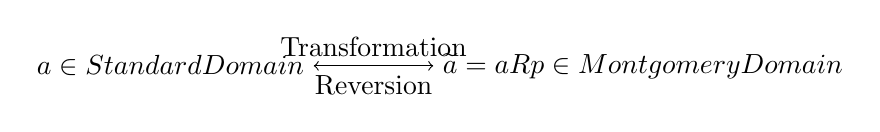
\begin{tikzpicture}
		\node (A) at (0,0) {$a \in \text{Standard Domain}$};
		\node (B) at (6,0) {$\widetilde{a} = aR \mod p \in \text{Montgomery Domain}$};
		\draw[->] (A) -- (B) node[midway,above] {Transformation};
		\draw[->] (B) -- (A) node[midway,below] {Reversion};
	\end{tikzpicture}
\end{center}

\newpage
\subsection{Montgomery Reduction}
Montgomery Reduction transforms the problem of modular multiplication into a more efficiently computable form by redefining the multiplication operation in terms of alternative representations of the numbers involved. Specifically, it introduces a mapping function based on a chosen constant $R$, which is co-prime to the modulus $m$ and typically a power of $2$ for computational efficiency.
\vspace{8pt}
\begin{example}
Compute \[
5\cdot 7\bmod{17}
\] \begin{proof}[\sol]
Let $N=17$ and $R=2^5=32>17$. Then \begin{itemize}
	\item $R^{-1}=8$ since $R^{-1}R=256\equiv 1\pmod{17}$;
	\item $N^{-1}=17$ since $N^{-1}N=289\equiv 1\pmod{32}$;
	\item $N'=R-N^{-1}=15$.
\end{itemize} 
\begin{itemize}
\item[] \textbf{Step 1: Transformation to Montgomery Space}

We transform $a=5$ and $b=7$ into Montgomery space: \begin{align*}
\tilde{a}&=5\cdot R\bmod 17\\
&=5\cdot32\bmod 17 = 7, \\
\tilde{b}&=7\cdot R\bmod 17\\
&=7\cdot32\bmod 17 = 3.
\end{align*} Here, $\tilde{a}$ and $\tilde{b}$ are the Montgomery representations of $a$ and $b$, respectively.
\item[] \textbf{Step 2: Montgomery Multiplication}

\begin{enumerate}
	\item \textit{Compute the product:} \[
	\tilde{a}\times\tilde{b}=21.
	\]
\end{enumerate}

Note that $R^{-1}$ satisfies $RR^{-1}\equiv 1\pmod{11}$: \begin{align*}
	R^{-1}R=R^{-1}\cdot 2^4&\equiv 1\pmod{11} \\
	R^{-1}R=R^{-1}\cdot 5&\equiv 1\pmod{11}\quad\because 16\equiv 5\pmod{11} \\
	R^{-1}&\equiv 9\pmod{11}\quad\because 5\cdot 9\equiv 1\pmod{11} \\
\end{align*} 
We multiply $X'$ and $Y'$ but the result is in Montgomery form: for $Z'=X'Y'$, \[
Z'R^{-1}\bmod 11 = 8\cdot 9\bmod 11 = 6.
\]
\item[] \textbf{Step 3: Conversion Back from Montgomery Space}
\end{itemize}
\end{proof}
\end{example}
\vspace{8pt}
\begin{tcolorbox}[colframe=defcolor,title={\color{white}\bf The Montgomery Representation and the inverse Montgomery Transformation}]
\begin{definition}
The Montgomery representation of a finite field element $x\in\intco{0,N}$, \[
\fullfunction{M}{\Z_N}{\Z_N}{x}{(xR)\bmod N},
\] is a mapping from the standard representation to the Montgomery domain, where $R=2^k$ for some $k$, a constant such that $R\geq m$ $\gcd(R,m)=1$.

The inverse Montgomery transformation, \[
\fullfunction{M^{-1}}{\Z_N}{\Z_N}{u}{(uR^{-1})\bmod N},
\] is a mapping back form the Montgomery domain to the standard representation, where $R^{-1}$ is the modular inverse of $R$ modulo $m$, \ie, $RR^{-1}\equiv 1\pmod{m}$.
\end{definition}
\end{tcolorbox}

\newpage
\begin{tcolorbox}[colframe=defcolor,title={\color{white}\bf The Montgomery Reduction}]
\begin{definition}
Define a mapping \textbf{Montgomery Reduction} $\mathsf{MontRed}:\Z_{NR}\to\Z_{N}$ as follows: \[
\mathsf{MontRed}(x):=xR^{-1}\bmod N,
\] for $x\in\intco{0,NR}$, where \begin{enumerate}[(i)]
\item $R=2^{wt}>N$
\item $\gcd(R=2^{wt}, N)=1$.
\end{enumerate}
\end{definition}	
\end{tcolorbox}
\begin{itemize}
	\item Let \( \mathcal{M} : \mathbb{F}_p \to \widetilde{\mathbb{F}}_p \) be the Montgomery transformation function, where \( \mathcal{M}(a) = aR \mod p \) transforms an element from the standard domain \( \mathbb{F}_p \) to the Montgomery domain \( \widetilde{\mathbb{F}}_p \).
	\item Let \( \mathcal{M}^{-1} : \widetilde{\mathbb{F}}_p \to \mathbb{F}_p \) be the inverse Montgomery transformation function, where \( \mathcal{M}^{-1}(\widetilde{a}) = \widetilde{a}R^{-1} \mod p \) transforms an element back from the Montgomery domain \( \widetilde{\mathbb{F}}_p \) to the standard domain \( \mathbb{F}_p \).
\end{itemize}

\newpage
\section{Montgomery Reduction}

\begin{tcolorbox}[colframe=defcolor,title={\color{white}\bf Montgomery From}]
\begin{definition}
Consider a element of finite field $\F_N$: \[
x\in\intco{0,N}.
\] Montgomery representation is defined as: \[
[x]:=(xR)\bmod N,
\] where \begin{enumerate}[(i)]
\item $R=2^{wt}>N$
\item $\gcd(R=2^{wt}, N)=1$.
\end{enumerate}
\end{definition}	
\end{tcolorbox}

\begin{tcolorbox}[colframe=defcolor,title={\color{white}\bf Montgomery Reduction}]
\begin{definition}
Define a mapping \textbf{Montgomery Reduction} $\mathsf{MontRed}:\Z_{NR}\to\Z_{N}$ as follows: \[
\mathsf{MontRed}(u):=uR^{-1}\bmod N,
\] for $u\in\set{[u]: u\in \F_N}$.
\end{definition}	
\end{tcolorbox}
\begin{remark}
\ \begin{itemize}
\item $\MontRed (xR^2\bmod N)=[x]$
\item $\MontRed ([x])=x$
\end{itemize}
\end{remark}

\begin{algorithm}[H]
\DontPrintSemicolon
\caption{Montgomery Reduction: $\MontRed(x)=x{2^{wt}}^{-1}\bmod N$}
\BlankLine
\Comment{${2^{wt}}^{-1}$ satisfies ${2^{wt}}{2^{wt}}^{-1}\equiv 1\pmod N$}
\Comment{$N^{-1}$ satisfies $NN^{-1}\equiv 1\pmod {2^{wt}}$}
\Comment{$N'$ satisfies $N'={2^{wt}}-N^{-1}$}
\KwIn{$(x{2^{wt}})\bmod N$ with the pre-computed values ${2^{wt}}$, $N'$}
\KwOut{$\MontRed(x)=x{2^{wt}}^{-1}\bmod N$}
\BlankLine
$s\gets(x\bmod {2^{wt}})\cdot N'\bmod {2^{wt}}$\tcp*{$s\gets (x\land \one^{wt})\cdot N^{-1}\bmod {2^{wt}}$}
$t\gets(x+s\cdot N) / {2^{wt}}$\tcp*{$t\gets (x+sN)\gg wt$ and then $t\in\intco{0,2N}$}
\If{$t\geq N$}{
	$t\gets t-N$
} \Return $t$\;
\end{algorithm}
\begin{proof}[Correctness for Montogmery Reduction]
\begin{align*}
s&=(x\bmod {2^{wt}})\cdot N'\bmod {2^{wt}}, \\
s&\equiv(x\bmod {2^{wt}})\cdot N'\pmod {2^{wt}}\\
&\implies\\
sN&\equiv(x\bmod {2^{wt}})\cdot N'N\pmod {2^{wt}}, \\
&\equiv (x\bmod {2^{wt}})(-N^{-1})N\pmod {2^{wt}}, \\
&\equiv -x\pmod{2^{wt}}\\
&\implies\\ 
&2^{wt}\mid sN-(-x)=sN+x\\
&\implies\\ 
&\frac{x+sN}{2^{wt}}\in\Z.
\end{align*}
\end{proof}

